\begin{figure}
  \centering
  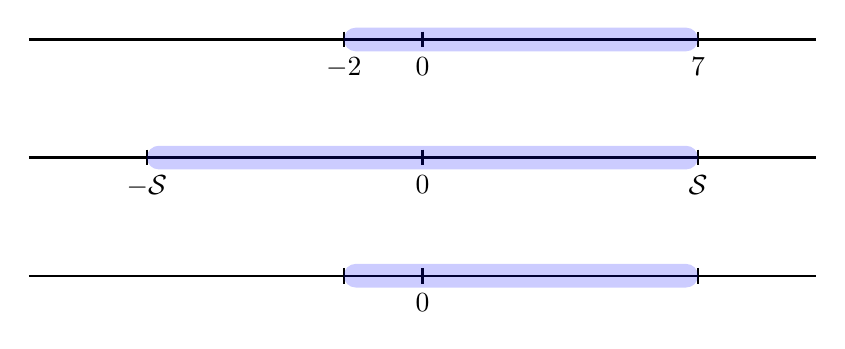
\begin{tikzpicture}[scale=0.5]
    \foreach \y/\lvalue/\uvalue/\llabel/\ulabel in {
      6/-2/7/$-2$/$7$,
      3/-7/7/$-\mathcal{S}$/$\mathcal{S}$,
      0/-2/7/$\LSize$/$\USize$
    } {
      \draw[-, thick] (-10,\y) -- (10,\y);
      \draw[thick] (0,\y+0.2) -- (0,\y-0.2) node[below] {0};
      \draw[thick] (\lvalue,\y+0.2) -- (\lvalue,\y-0.2) node[below] {\llabel};
      \draw[thick] (\uvalue,\y+0.2) -- (\uvalue,\y-0.2) node[below] {\ulabel};
      \fill[opacity=0.2,blue,rounded corners=1ex] (\lvalue,\y-0.3) -- (\uvalue,\y-0.3) -- (\uvalue,\y+0.3) -- (\lvalue,\y+0.3) -- cycle;
    }
  \end{tikzpicture}
\end{figure}
